
\section{Introduction}
Clustering is the prototypical unsupervised learning activity which consists of identifying cohesive and well-differentiated groups of records in data. It aims to partition a set of objects such that similar objects will be assigned to the same group while those that are dissimilar will be placed in different groups~\cite{jain2010data}. 

\lipsum[2-4]
\lipsum[2-4]

\lipsum[2-4]
% insert figure here
\begin{figure}[!ht]
\centering
\begin{subfigure}[b]{0.45\textwidth}
                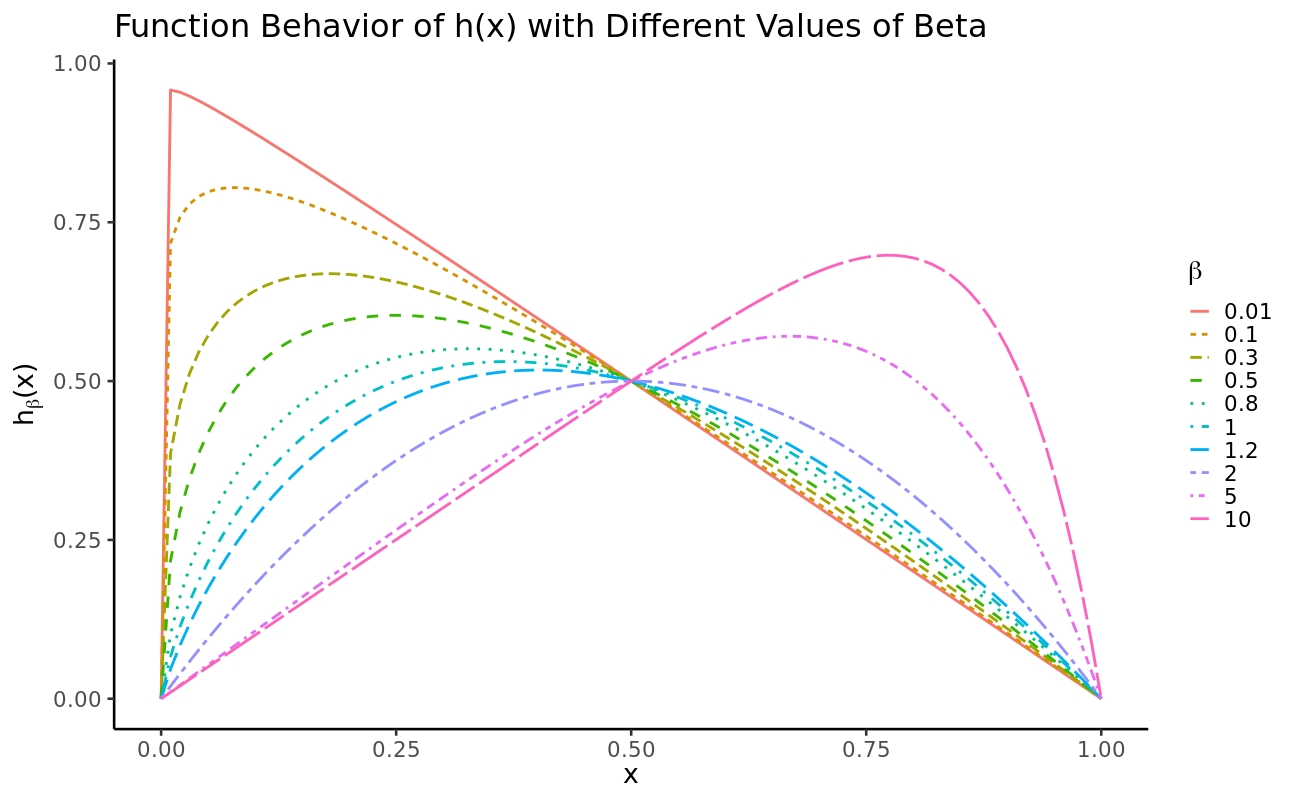
\includegraphics[width=\textwidth]{graph/betaFuncBehv.jpeg}
                \caption{\textit{Partition with 2 clusters.}}
                \label{fig:prt5cls_2clst}
\end{subfigure}
\begin{subfigure}[b]{0.45\textwidth}
                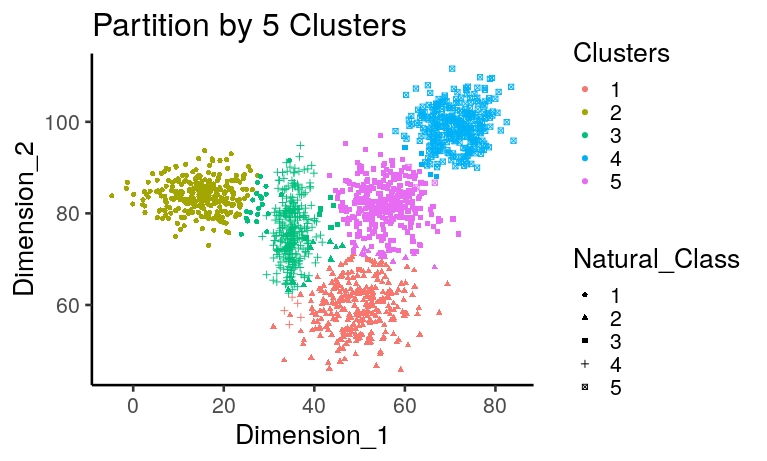
\includegraphics[width=\textwidth]{graph/prt5cls_5clst.jpeg}
                \caption{\textit{Partition with 3 clusters.}}
                \label{fig:prt5cls_3clst}
\end{subfigure}\\
\caption{Test figure.}
\label{fig:prt5cls}
\end{figure}

\section{Test section}
\lipsum[2-4]

\lipsum[2-4]

\lipsum[2-4]


 